\section{Executing COMPSs applications}
\label{sec:Executing}


\subsection{Prerequisites}
\label{subsec:prerequisites}
Prerequisites vary depending on the application's code language: for Java applications the users need to have
a \textbf{jar archive} containing all the application classes, for Python applications there are no requirements and for
C/C++ applications the code must have been previously compiled by using the \textit{buildapp} command.

For further information about how to develop applications for COMPSs please refer to the \textit{COMPSs User 
Manual: Application development guide} available at the \url{http://compss.bsc.es/} webpage.


\subsection{Runcompss command}
\label{subsec:runcompss}
All COMPSs applications are executed using the \textbf{runcompss} command which is invoked as follows:
\begin{lstlisting}[language=bash]
compss@bsc:~$ runcompss [options] application_name [application_arguments]
\end{lstlisting}

The application name stands for the fully qualified name of the application in Java, for the path to the \textit{.py} file
containing the main program in Python and for the path to the master binary in C/C++. 

The application arguments are the arguments that the users' main application recieves. If needed, they can be empty. 

The runcompss command allows the users to customize each COMPSs execution by specifying different options.
For clarity purposes, parameters are grouped in \textit{Runtime configuration}, \textit{Tools enablers}
and \textit{Advanced options}. Users can add any of them to the runcompss call by following the next 
usage description.

\begin{lstlisting}[language=bash]
compss@bsc:~$ runcompss -h
  Runtime configuration options:
    - -project=<path>                       Path to the project XML file
                                            Default: /opt/COMPSs/Runtime/configuration/
                                            xml/projects/project.xml
                                            
    - -resources=<path>                     Path to the resources XML file
                                            Default: /opt/COMPSs/Runtime/configuration/
                                            xml/resources/resources.xml
                                            
    - -lang=<name>                          Language of the application (java/c/python)
                                            Default: java
                                            
    - -log_level=<level>, - -debug, -d      Set the debug level: off | info | debug
                                            Default: off

  Tools enablers:
    - -graph=<bool>, - -graph, -g           Generation of the complete graph (true/false)
                                            When no value is provided it is set to true
                                            Default: false
                                            
    - -tracing=<bool>, - -tracing, -t       Generation of traces (true/false)
                                            When no value is provided it is set to true
                                            Default: false
                                            
    - -monitoring=<int>, - -monitoring, -m  Period between monitoring samples 
                                            (milliseconds)
                                            When no value is provided it is set to 2000
                                            Default: 0

  Advanced options:
    - -comm=<path>                          Class that implements the adaptor for 
                                            communications
                                            Default: integratedtoolkit.nio.master.
                                            NIOAdaptor
                                            
    - -library_path=<path>                  Non-standard directories to search for 
                                            libraries (e.g. Java JVM library, Python 
                                            library, C binding library) 
                                            Default: .
                                            
    - -classpath=<path>                     Path for the application classes / modules
                                            Default: .
                                            
    - -task_count=<int>                     Only for C/Python Bindings. 
                                            Maximum number of different functions/methods
                                            invoked from the application that have been 
                                            selected as tasks
                                            Default: 50
                                            
    - -uuid=<int>                           Preset an application UUID
                                            Default: Automatic random generation
\end{lstlisting}

\subsection{Running a COMPSs application}
\label{subsec:running_compss}
Before running COMPSs applications it is important to notice that the application files \textbf{must} be in the \textbf{CLASSPATH}.
Thus, when launching a COMPSs application, users can manually pre-set the \textbf{CLASSPATH} environment variable
or can add the \textit{- - classpath} option to the runcompss command.

The next three sections provide specific information for launching COMPSs applications in different code languages (Java, Python and 
C/C++). For clarity purposes we will use the \textit{Simple} application (developed in Java, Python and C++) available at our
Virtual Machine or at \url{https://compss.bsc.es/projects/bar} webpage. This application takes an integer as input
parameter and increases it by one unit using a task. For further details about the codes please refer to the \textit{Sample 
Applications} document available at \url{http://compss.bsc.es} .

\subsubsection{Running Java applications}
A Java COMPSs application can be launched through the following command:
\begin{lstlisting}[language=bash]
compss@bsc:~$ cd workspace_java/simple/jar/
compss@bsc:~/workspace_java/simple/jar$ runcompss simple.Simple <initial_number>
\end{lstlisting}

\begin{figure}[h!]
  \centering
    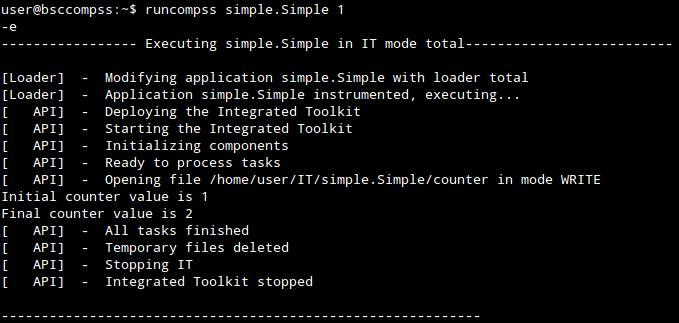
\includegraphics[width=\textwidth]{./Sections/2_Execution/Figures/java_execution.jpeg}
    \caption{Execution of a Java COMPSs application.}
    \label{fig:java_execution}
\end{figure}
\vspace{-0.4cm}

In this first execution we are taking advantage of the default value of the - -classpath option to automatically add the jar
file to the classpath (by moving to the directory which contains the jar file before launching the COMPSs application). However,
we can explicitly do this by exporting the \textbf{CLASSPATH} variable or by providing the 
- -classpath value. Next, we provide another two ways to perform the same execution:

\begin{lstlisting}[language=bash]
compss@bsc:~$ export CLASSPATH=$CLASSPATH:
                               /home/compss/workspace_java/simple/jar/simple.jar
compss@bsc:~$ runcompss simple.Simple <initial_number>
\end{lstlisting}

\begin{lstlisting}[language=bash]
compss@bsc:~$ runcompss --classpath=/home/compss/workspace_java/simple/jar/simple.jar 
                        simple.Simple <initial_number>
\end{lstlisting}


\subsubsection{Running Python applications}
To lauch a Python application with COMPSs users only need to provide the \textit{- -lang=python} option to the runcompss command. 
Next, we provide an example of a simple python application.

\begin{lstlisting}[language=bash]
compss@bsc:~$ cd workspace_python/simple/
compss@bsc:~/workspace_python/simple$ runcompss --lang=python simple.py <initial_number>
\end{lstlisting}

\begin{figure}[h!]
  \centering
    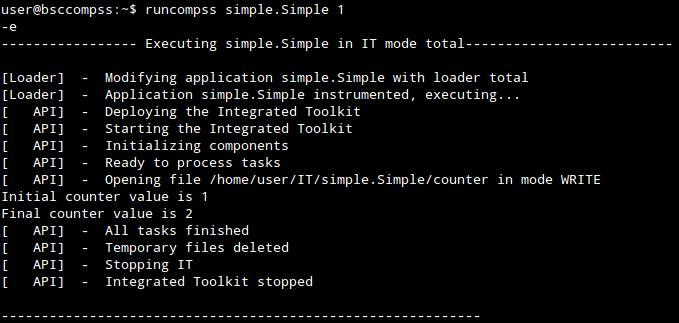
\includegraphics[width=\textwidth]{./Sections/2_Execution/Figures/python_execution.jpeg}
    \caption{Execution of a Python COMPSs application.}
    \label{fig:python_execution}
\end{figure}
\vspace{-0.4cm}


\subsubsection{Running C/C++ applications}
To lauch a C/C++ application with COMPSs users need to compile the C/C++ application by using the \textit{buildapp} command. For 
further information please refer to the \textit{COMPSs User Manual: Application development guide} document available at our
webpage \url{http://compss.bsc.es} . Once done, to run the C/C++ application with COMPSs, the users only need to provide 
the \textit{--lang=c} option to the runcompss command. Next, we provide an example of a simple C++ application:

\begin{lstlisting}[language=bash]
compss@bsc:~$ cd workspace_c/simple/
compss@bsc:~/workspace_c/simple$ runcompss --lang=c simple <initial_number>
\end{lstlisting}

\begin{figure}[h!]
  \centering
    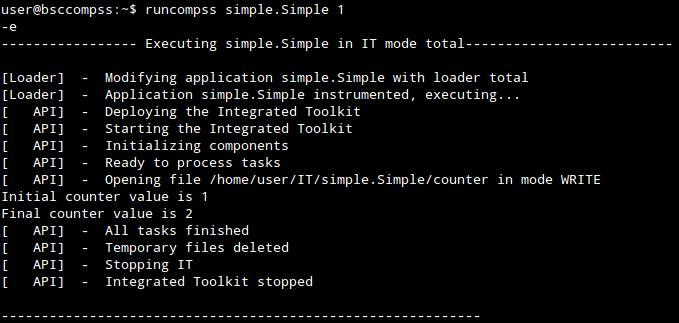
\includegraphics[width=0.95\textwidth]{./Sections/2_Execution/Figures/c_execution.jpeg}
    \caption{Execution of a C++ COMPSs application.}
    \label{fig:c_execution}
\end{figure}
\vspace{-0.4cm}


\subsection{Additional configurations}

COMPSs has \textbf{two} configuration files: \textit{resources.xml} and \textit{project.xml} . 
These files are meant to provide information about the execution environment 
and are completely independent from the application.

For each execution users can load the default configuration files or specify their custom configurations 
by using, respectively, the \textit{$--resources=<absolute\_path\_to\_resources.xml>$} and the
\textit{$--project=<absolute\_path\_to\_project.xml>$} inside the \textit{runcompss} command. The default files are located 
under the \emph{/opt/COMPSs/Runtime/configuration/xml/} path. 
Users can edit these two files manually or can take advantage of the \textit{Eclipse IDE} tool developed for COMPSs. For further 
information about the \textit{Eclipse IDE} please refer to Section \ref{subsec:IDE}. 


Next sections provide more in-depth information about the \textit{resources.xml} and the \textit{project.xml} files, listing and 
explaining the available tags.

\subsubsection{Resources file}
The resources file provides information about \textbf{all} the available resources. This file should normally be 
managed by the system administrators. Its full definition schema can be found at 
\emph{/opt/COMPSs/Runtime/configuration/xml/resources/$resource_schema$.xsd}.

The typical strcuture of this file is one entry per available resource defining its name, its capabilities and its requirements.
Administrators can define several resource capabilities (see example in next listing) but we would like 
to underline the importance of \textbf{Processor CoreCount}. This capability represents the number of available cores 
in the resource and it is used to schedule the correct number of tasks into a resource. Thus, it becomes essential to define 
it accordingly to the number of cores in the physical resource. 

\begin{lstlisting}[language=xml]
compss@bsc:~$ cat /opt/COMPSs/Runtime/configuration/xml/resources/resources.xml
<?xml version="1.0" encoding="UTF-8"?>
<ResourceList>
        <Resource Name="localhost">
                <Capabilities>
                        <Host>
                                <TaskCount>0</TaskCount>
                                <Queue>short</Queue>
                                <Queue/>
                        </Host>
                        <Processor>
                                <Architecture>IA32</Architecture>
                                <Speed>3.0</Speed>
                                %*{\bf $<CoreCount>4</CoreCount>$ }*)
                        </Processor>
                        <OS>
                                <OSType>Linux</OSType>
                                <MaxProcessesPerUser>32</MaxProcessesPerUser>
                        </OS>
                        <StorageElement>
                                <Size>8</Size>
                        </StorageElement>
                        <Memory>
                                <PhysicalSize>4</PhysicalSize>
                                <VirtualSize>8</VirtualSize>
                        </Memory>
                        <ApplicationSoftware>
                                <Software>Java</Software>
                        </ApplicationSoftware>
                        <Service/>
                        <VO/>
                        <Cluster/>
                        <FileSystem/>
                        <NetworkAdaptor/>
                        <JobPolicy/>
                        <AccessControlPolicy/>
                </Capabilities>
                <Requirements/>
        </Resource>
</ResourceList>
\end{lstlisting}


\subsubsection{Project file}
The project file provides specific execution information. Particullarly, it selects and configures in which resources
is the application going to be executed. Consequently, the resources that appear in this file are a \textbf{subset} of the 
resources described in the \textit{resources.xml} file. This file should normally be managed by the application users and will
usally change from execution to execution. Its full definition schema can be found at 
\emph{/opt/COMPSs/Runtime/configuration/xml/projects/$project_schema$.xsd}.

The typical strcuture of this file is one entry per worker, indicating the the resource name that it uses and some configuration
properties (see example in next listing). We emphasize the importance of correctly defining the following 
entries:
\begin{description}
 \item [installDir] Indicates the path of the COMPSs installation \textbf{inside the resource} (not necessarily the same 
 than in the local machine).
 \item [User] Indicates the username used to connect via ssh to the resource. This user \textbf{must} have passwordless access to the
 resource (for more information check the \textit{COMPSs Installation Manual} available at our website \url{http://compss.bsc.es}).
 If left empty COMPSs will automatically try to access the resource with the \textbf{same username than the one that lauches 
 the COMPSs main application}.
 \item [LimitOfTasks] The maximum number of tasks that can be simultaneously scheduled to a resource. Considering that a task 
 can use more than one core but not least, this value must be lower or equal to the number of available cores in the resource. 
\end{description}


\begin{lstlisting}[language=xml]
compss@bsc:~$ cat /opt/COMPSs/Runtime/configuration/xml/projects/project.xml
<?xml version="1.0" encoding="UTF-8"?>
<Project>
	<!--Description for any physical node-->
	<Worker Name="localhost">
		%*{\bf $<InstallDir>/opt/COMPSs/Runtime/scripts/system/</InstallDir>$ }*)
		<WorkingDir>/tmp/</WorkingDir>
		%*{\bf $<!-- <User>user</User> -->$ }*)
		%*{\bf $<LimitOfTasks>4</LimitOfTasks>$ }*)
	</Worker>
</Project>
\end{lstlisting}
\label{lstlisting:project.xml}


\subsection{Configuration examples}
In the next subsections we provide specific information about the services, shared disks, cluster and cloud configurations. 
Moreover there are \textit{project.xml} and \textit{resources.xml} examples for each case that can be used as templates. 


\subsubsection{Services configuration example}
To allow COMPSs applications use WebServices the \textit{resources.xml} can include a special type of resource called 
\textit{Service}. For each WebService it is necessary to specify its wsdl, its name, its namespace and
its port as shown in the following example. 
\begin{lstlisting}[language=xml]
<?xml version="1.0" encoding="UTF-8"?>
<ResourceList>
        <Resource Name="localhost">
                ...
        </Resource>
                
        <Service wsdl="http://bscgrid05.bsc.es:20390/hmmerobj/hmmerobj?wsdl">
                <Name>HmmerObjects</Name>
                <Namespace>http://hmmerobj.worker</Namespace>
                <Port>HmmerObjectsPort</Port>
        </Service>
</ResourceList>
\end{lstlisting}

When configuring the \textit{project.xml} file it is necessary to include the service as a worker by adding an
special entry indicating only the name and the limit of tasks as shown in the following example:
\begin{lstlisting}[language=xml]
<?xml version="1.0" encoding="UTF-8"?>
<Project>
        <!--Description for any physical node-->
        <Worker Name="localhost">
               ...
        </Worker>

        <Worker Name="http://bscgrid05.bsc.es:20390/hmmerobj/hmmerobj?wsdl">
               <LimitOfTasks>3</LimitOfTasks>
        </Worker>
</Project>
\end{lstlisting}

\subsubsection{Cluster configuration (static resources) example}
In order to use external resources to execute the applications, the following steps have to be followed:

\begin{enumerate}
 \item Install the \textit{COMPSs Worker} package (or the full \textit{COMPSs Framework} package) on all the new 
 resources following the \textit{Installation manual} available at \url{http://compss.bsc.es} .
 \item Set SSH passwordless access to the rest of the remote resources.
 \item Create the \textit{WorkingDir} directory in the resource (remember this path because it is needed 
 for the \textit{project.xml} configuration).
 \item Deploy the application manually on each resource.
\end{enumerate}

Once these steps are done, users need to configure the \textit{resources.xml} and the \textit{project.xml} files accordingly.
On the following lines, we provide examples about configuration files for Grid and Cluster environments, 
which can serve as a reference

\begin{lstlisting}[language=xml]
<?xml version="1.0" encoding="UTF-8" standalone="yes"?>
<ResourceList>
    <Resource Name="hostname1.domain.es">
        <Capabilities>
            <Host>
                <TaskCount>0</TaskCount>
                <Queue>Short</Queue>
            </Host>
            <Processor>
                <Architecture>x86_64</Architecture>
                <Speed>2.5</Speed>
                <CoreCount>4</CoreCount>
            </Processor>
            <OS>
                <OSType>Linux</OSType>
            </OS>
            <StorageElement>
                <Size>250.0</Size>
            </StorageElement>
            <Memory>
                <PhysicalSize>4.0</PhysicalSize>
            </Memory>
            <ApplicationSoftware>
                <Software>BLAST</Software>
            </ApplicationSoftware>
        </Capabilities>
        <Disks/>
    </Resource>
    <Resource Name="hostname2.domain.es">
	...
    </Resource>
</ResourceList>
\end{lstlisting}

\begin{lstlisting}[language=xml]
<?xml version="1.0" encoding="UTF-8" standalone="yes"?>
<Project>
    <Worker Name="hostname1.domain.es">
        <InstallDir>/opt/COMPSs/Runtime/scripts/system/</InstallDir>
        <WorkingDir>/home/user/</WorkingDir>
        <User>user</User>
        <LimitOfTasks>2</LimitOfTasks>
    </Worker>
    <Worker Name="hostname2.domain.es">
        ...
    </Worker>
</Project>
\end{lstlisting}


\subsubsection{Shared Disks configuration example}
Configuring shared disks might reduce the amount of data transfers improving the application performance. To configure a 
shared disk the users must edit the \textit{resources.xml} indicating how the shared disk is hosted in the master node 
and how the shared disk is mounted in each worker. 

To indicate a shared disk hosted in the master node the \textit{resources.xml} file must include a \textit{Disk} tag describing
the disk and the mount point. The following example states that in the master node there is a shared disk labelled 
\textit{sharedDisk0} mounted on the \textit{/sharedDisk} directory.
\begin{lstlisting}[language=xml]
<?xml version="1.0" encoding="UTF-8"?>
<ResourceList>
    <Disk Name="sharedDisk0">
        <MountPoint>/sharedDisk</MountPoint>
    </Disk>
<ResourceList>
\end{lstlisting}

On the other side, to declare that a worker has a shared disk mounted the \textit{resources.xml} file must include a \textit{Disk}
tag inside the specific worker indicating its name (defined in the master \textit{Disk} tag) and its mount point inside the worker.
The following example states that the \textit{sharedDisk0} is mounted on resource \textit{hostname1.domain.es} under the path
\textit{/home/user/mySharedDisk/} .
\begin{lstlisting}[language=xml]
<Resource Name="hostname1.domain.es">
    <Capabilities>
    ...
    </Capabilities>
    <Requirements/>
    <Disks>
        <Disk Name="sharedDisk0">
            <MountPoint>/home/user/mySharedDisk</MountPoint>
        </Disk>
    </Disks>
</Resource>
\end{lstlisting}

Although, the example only contains the definition of a single shared disk, the \textit{Disks} tag can have multiple 
disk child nodes.


\subsubsection{Cloud configuration (dynamic resources) example}
In order to use cloud resources to execute the applications, the following steps have to be followed:
\begin{enumerate}
 \item Prepare cloud images with the \textit{COMPSs Worker} package or the full \textit{COMPSs Framework} package installed.
 \item The application will be deployed automatically during execution but the users need to set up the configuration files to
 specify the application files that must be deployed. 
\end{enumerate}

The COMPSs runtime communicates with the Cloud by means of Cloud connectors. Each connector implements 
the interaction of the runtime with a given Cloud provider, more precisely by supporting four basic 
operations: ask for the price of a certain VM in the provider, get the time needed to create a VM, 
create a new VM and terminate a VM. This design allows connectors to abstract the runtime from the particular API
of each provider and facilitates the addition of new connectors for other providers.

In order to add cloud resources the \textit{resources.xml} file can contain one or more \textbf{$<CloudProvider>$} tags
that encompass the information about a particular Cloud provider, associated to a given connector. The tag \textbf{must} have an
attribute \textbf{name} to uniquely identify the provider. Table \ref{tab:conf_resources_xml} summarizes the information to be 
specified by the user inside this tag.

\begin{longtable}{| p{0.45\textwidth} | p{0.45\textwidth} |}
\hline
Server			&		Endpoint of the provider’s server	\\
\hline
Connector		&		Class that implements the connector	\\
\hline
\textbf{
ImageList
\begin{itemize}
 \item Image
 \begin{itemize}
  \item Architecture
  \item OSType
  \item ApplicationSoftware
  \begin{itemize}
   \item Software
  \end{itemize}
  \item SharedDisks
  \begin{itemize}
   \item Disk
  \end{itemize}
 \end{itemize}
\end{itemize}
}
&
Multiple entries of VM templates
\begin{itemize}
 \item VM image
 \begin{itemize}
  \item Architeture of the VM image
  \item Operative System installed in the VM image
  \item Multiple entries of software installed in the VM image
  \begin{itemize}
   \item Software installed in the VM image
  \end{itemize}
  \item Multiple entries of shared disks mounted in the VM image
  \begin{itemize}
   \item Disk description
  \end{itemize}
 \end{itemize}
\end{itemize}
\\
\hline

\textbf{
InstanceTypes
\begin{itemize}
 \item Resource
 \begin{itemize}
  \item Capabilities
  \begin{itemize}
   \item Processor
   \item StorageElement
   \item Memory
  \end{itemize}
 \end{itemize}
\end{itemize}
}
& 
Multiple entries of resource templates
\begin{itemize}
 \item Instance type offered by the provider
 \begin{itemize}
  \item Hardware details of instance type
  \begin{itemize}
   \item Architecture and number of available cores
   \item Size in GB of the storage
   \item PhysicalSize, in GB of the available RAM
  \end{itemize}
 \end{itemize}
\end{itemize}
\\
\hline

\caption{Configuration of resources.xml file, tag $<CloudProvider>$}
\label{tab:conf_resources_xml}
\end{longtable}

The \textit{project.xml} complements the information about Cloud providers specified in the \textit{resources.xml} file. 
This file can contain a \textbf{$<Cloud>$} tag where to specify a list of providers, each with a \textbf{$<Provider>$} tag,
whose \textbf{name} attribute must match one of the providers in the \textit{resources.xml} file. Thus, the \textit{project.xml}
file \textbf{must} contain a subset of the providers specified in the \textit{resources.xml} file. Table 
\ref{tab:conf_project_xml_provider} summarizes the information that users need to specify inside the \textbf{$<Cloud>$} tag and
Table \ref{tab:conf_project_xml_cloud} summarizes the information that users need to specify inside the \textbf{$<Provider>$} 
tag of the \textit{project.xml} file.

\begin{table}[h]
  \begin{center}
    \begin{tabular}{| p{0.45\textwidth} | p{0.45\textwidth} |}
      \hline
      InitialVMs	&	Number of VM to be created at the beginning of the application	\\
      \hline
      minVMCount	&	Minimum number of VMs available in the computation	\\
      \hline
      maxVMCount	&	Maximum number of VMs available in the computation	\\
      \hline
      Provider 	&	Multiple entries of Cloud providers	\\
      \hline
    \end{tabular}
    \caption{Configuration of project.xml file, tag $<Cloud>$}
    \label{tab:conf_project_xml_cloud}
  \end{center}
\end{table}

\newpage

\begin{longtable}{| p{0.43\textwidth} | p{0.57\textwidth} |}
  \hline
  LimitOfVMs	&	Maximum number of VMs allowed by the provider	\\
  
  \hline
  Property
  \begin{itemize}
    \item Name
    \item Value
  \end{itemize}
  &
  Multiple entries of provider-specific properties
  \begin{itemize}
    \item Name of the property
    \item Value of the property
  \end{itemize}
  \\
  \hline
  
  ImageList
  \begin{itemize}
  \item Image
  \begin{itemize}
    \item InstallDir
    \item WorkingDir
    \item User
    \item Package
    \begin{itemize}
    \item Source
    \item Target
    \item InstalledSoftware
    \end{itemize}
  \end{itemize}
  \end{itemize}
  & 
  Multiple entries of VM images available at the provider
  \begin{itemize}
    \item VM image
    \begin{itemize}
      \item Path of the COMPSs worker scripts in the image
      \item COMPSs working directory in the deployed instances
      \item Account username
      \item Multiple entries of local packages that have to be deployed in new instances
      \begin{itemize}
	\item Local path of the package
	\item Path where to deploy the package in the new instance
	\item List of software included in the package
      \end{itemize}
    \end{itemize}
  \end{itemize}
  \\
  \hline
  
  InstanceTypes
  \begin{itemize}
  \item Resource
  \end{itemize}
  & 
  List of resource types that are available in the provider
  \begin{itemize}
  \item Resource description
  \end{itemize}
  \\
  \hline
  
  \caption{Configuration of project.xml file, tag $<Provider>$}
  \label{tab:conf_project_xml_provider}
\end{longtable}

The next sections provide a description of each of the currently available connector.

\newpage

\paragraph{Cloud connectors: Amazon EC2}
The COMPSs runtime features a connector to interact with the Amazon Elastic Compute Cloud (EC2).

Amazon EC2 offers a well-defined pricing system for VM rental. A total of 8 pricing zones are 
established, corresponding to 8 different locations of Amazon datacenters around the globe. 
Besides, inside each zone, several per-hour prices exist for VM instances with different capabilities. 
The EC2 connector stores the prices of standard on-demand VM instance types (t1.micro, m1.small, 
m1.medium, m1.large and m1.xlarge) for each zone. Spot instances are not currently supported by the connector.

When the COMPSs runtime chooses to create a VM in the Amazon public Cloud, the EC2 connector receives 
the information about the requested characteristics of the new VM, namely the number of cores, memory, 
disk and architecture (32/64 bits). According to that information, the connector tries to find the VM 
instance type in Amazon that better matches those characteristics and then requests the creation of a 
new VM instance of that type.

Once an EC2 VM is created, a whole hour slot is paid in advance; for that reason, the connector keeps 
the VM alive at least during such period, saving it for later use if necessary. When the task load 
decreases and a VM is no longer used, the connector puts it aside if the hour slot has not expired yet, 
instead of terminating it. After that, if the task load increases again and the EC2 connector requests 
a VM, first the set of saved VMs is examined in order to find a VM that is compatible with the requested 
characteristics. If one is found, the VM is reused and becomes eligible again for the execution of tasks; 
hence, the cost and time to create a new VM are not paid. A VM is only destroyed when the end of its hour 
slot is approaching and it is still in saved state.

Table \ref{tab:conf_project_xml_provider} summarizes the provider-specific properties that must be 
defined in the project.xml file for the Amazon EC2 connector.

\begin{longtable}{| p{0.3\textwidth} | p{0.7\textwidth} |}
\hline
{\bf Placement }    &   Location of the amazon datacentre to use \\
\hline
Access Key Id       &   Identifier of the access key of the Amazon EC2 account \\
\hline
Secret Key Id       &   Identifier of the secret key of the Amazon EC2 account \\
\hline
Key host location   &   Path to the SSH key in the local host, used to connect to the VMs \\
\hline
KeyPair name        &   Name of the key pair to use \\
\hline
SecurityGroup name  &   Name of the security group to use \\
\hline
\caption{Properties of the Amazon EC2 connector.}
\label{tab:ec2_connector_properties}
\end{longtable}

\paragraph{Cloud connectors: rOCCI}
In order to execute a COMPSs application in the cloud, the rOCCI connector has to be configured properly. 
The connector uses the rOCCI binary client\footnote{\url{https://appdb.egi.eu/store/software/rocci.cli}} 
(version newer or equal than 4.2.5) which has to be installed in the node where the COMPSs main 
application is executed.

This connector needs additional files providing details about the resource templates available on 
each provider. This file is located under $<COMPSs\_INSTALL\_DIR>/configuration/xml/templates$ path. 
Additionally, the user must define the virtual images flavour and instance types offered by each provider; 
thus, when the runtime asks for the creation of a VM, the connector selects the appropriate image and 
resource template according to the requirements (in terms of CPU, memory, disk, etc) by invoking the 
rOCCI client through Mixins (heritable classes that override and extend the base templates).

Table \ref{tab:rOCCI_extensions} contains the rOCCI specific properties that must be defined in the 
project.xml file.

\begin{longtable}{| p{0.25\textwidth} | p{0.75\textwidth} |}
\hline
{\bf Provider }    &  \\
\hline
ca-path     &   Path to CA certificates directory \\
\hline
user-cred   &   Path of the VOMS proxy \\
\hline
auth        &   Authentication method, x509 only supported \\
\hline
owner & \multirow{2}{*}{Optional. Used by the VENUS-C Job Manager (PMES)} \\
\cline{1-1}
jobname &  \\
\hline
\caption{rOCCI extensions in the project.xml file.}
\label{tab:rOCCI_extensions}
\end{longtable}

\vspace{-0.75cm}

\begin{longtable}{| p{0.25\textwidth} | p{0.75\textwidth} |}
\hline
\textbf{Instance} 	& Multiple entries of resource templates. \\ \hline
Type   			&    Name of the resource template. It has to be the same name than in the previous files \\ \hline
CPU    			&    Number of cores \\ \hline
Memory 			&    Size in GB of the available RAM \\ \hline
Disk   			&    Size in GB of the storage \\ \hline
Price  			&    Cost per hour of the instance \\ \hline
\caption{Configuration of the $<provider>.xml$ templates file.}
\label{tab:rOCCI_configuration}
\end{longtable}
